Hiring effectively is one of the key challenge that any organization faces. There are, two possibly conflicting, optimization issues that a hiring committee faces (i) how well the new member can mingle to the existing members of the organization, (ii) how much of a value addition the new member makes to the organization. The first consideration is commonly known as the \textit{communication cost}. Whereas the second consideration is dependent on the tasks that organization is aiming to complete and the skill that a member has with respect to the task requirement. This is called \textit{coverage} in the team formation literature. 

Lappas et al. \citep{lappas2009finding} in their seminal paper first introduced the problem of \textit{team formation}, where they modelled a team in the form of a graph. They proposed two graph distance based measures of the communication cost, namely the diameter and minimum spanning tree of the graph. They showed that for both types of communication costs the team formation problem is NP-complete. Later in series of works \cite{sozio2010community,kargar2011discovering,anagnostopoulos2010power,rangapuram2013towards} more realistic team  formation problems has been explored. In \cite{bhowmik2014submodularity} the submodularity of the team formation problem is established which enabled better approximation of the faster greedy heuristics. However one key difference of all these works, in light of ours is that, we consider presence of a team already, unlike the other works where teams are being formed from scratch. Our problem thus better be viewed as a \textit{hiring problem}. Moreover the set of tasks is also unknown. In \cite{anagnostopoulos2012online} authors assume that tasks arrive in an online manner. Teams are formed that such that most of the tasks can be accomplished. In our problem we assume that a tasks are drawn from a known distribution. Thus the exact set of tasks has a probability associated with it. We want to hire candidates such that with high probability all the tasks of the distribution can be completed.

To understand this better, refer to figure \ref{fig:hpo}. Our problem has three inputs, an existing team, a pool of candidates and a task distribution. Our aim is to find a a candidate from the pool that maximizes the expected coverage while adding minimum communication overhead. 
\begin{figure}
\centering
\begin{small}
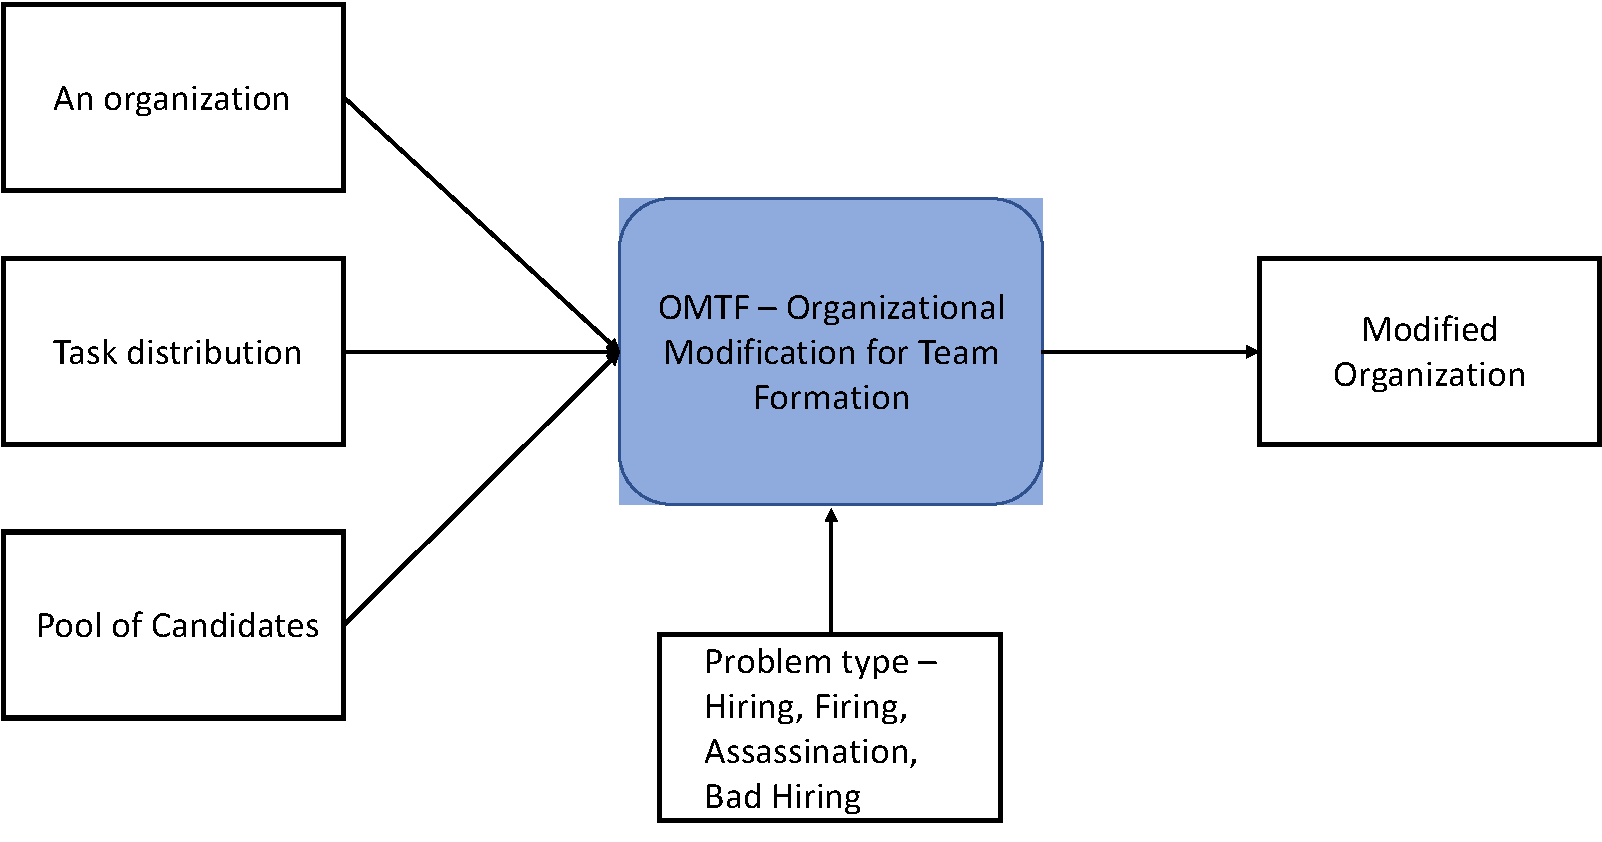
\includegraphics[width=.25\textwidth]{figs/pdf/illustration.pdf}
\caption{Hiring problem overview}
\label{fig:hpo}
\end{small}
\end{figure} 

In this paper we show that the hiring problem is NP-complete. However we provide two realistic communication and coverage functions such that both have submodular property. When those two functions are submodular, we can design a greedy approximation \cite{pmlr-v48-baib16} that preserves $1 - \frac{1}{e}$ - approximation. Thus to summarize our contributions are as follows:

\begin{enumerate}
\item We formulate the novel \textit{hiring problem}, which draws its inspiration from team formation literature.

\item We show that the problem is NP-hard. However under certain communication and coverage function, efficient approximation algorithm can be designed for the problem.

\item By lifting the algorithm of \cite{pmlr-v48-baib16}, we design a greedy algorithm that preserves $1 - \frac{1}{e}$ approximation ratio.

\item Through extensive experiments on both real world and synthetic datasets, we empirically show the superiority of our approach over existing baselines. 

\end{enumerate}